\subsubsection{22.12.14}
\begin{enumerate}
	
	\item Время начала и окончания собрания: 16:00 - 18:50.
	
	\item Цели собрания: 
	\begin{enumerate}
		
		\item Заменить сломаный привод (задний правый).
		
		\item Переделать внутреннюю часть откосов таким образом, чтобы мячи не застревали на них.
		
	\end{enumerate}

	\item Проделанная работа:
	\begin{enumerate}
		
		\item Привод был заменен, однако протестировать его мы не смогли, поскольку у нас не было доступного компьютера.
		
        \item Откосы были заменены. Во время испытаний откосы работали как нужно: возвращали мячи, попавшие на них, обратно в рабочую область захвата мячей.
		
        \begin{figure}[H]
	  	  \begin{minipage}[h]{0.2\linewidth}
	  	    \center  
	  	  \end{minipage}
	  	  \begin{minipage}[h]{0.6\linewidth}
	  		\center{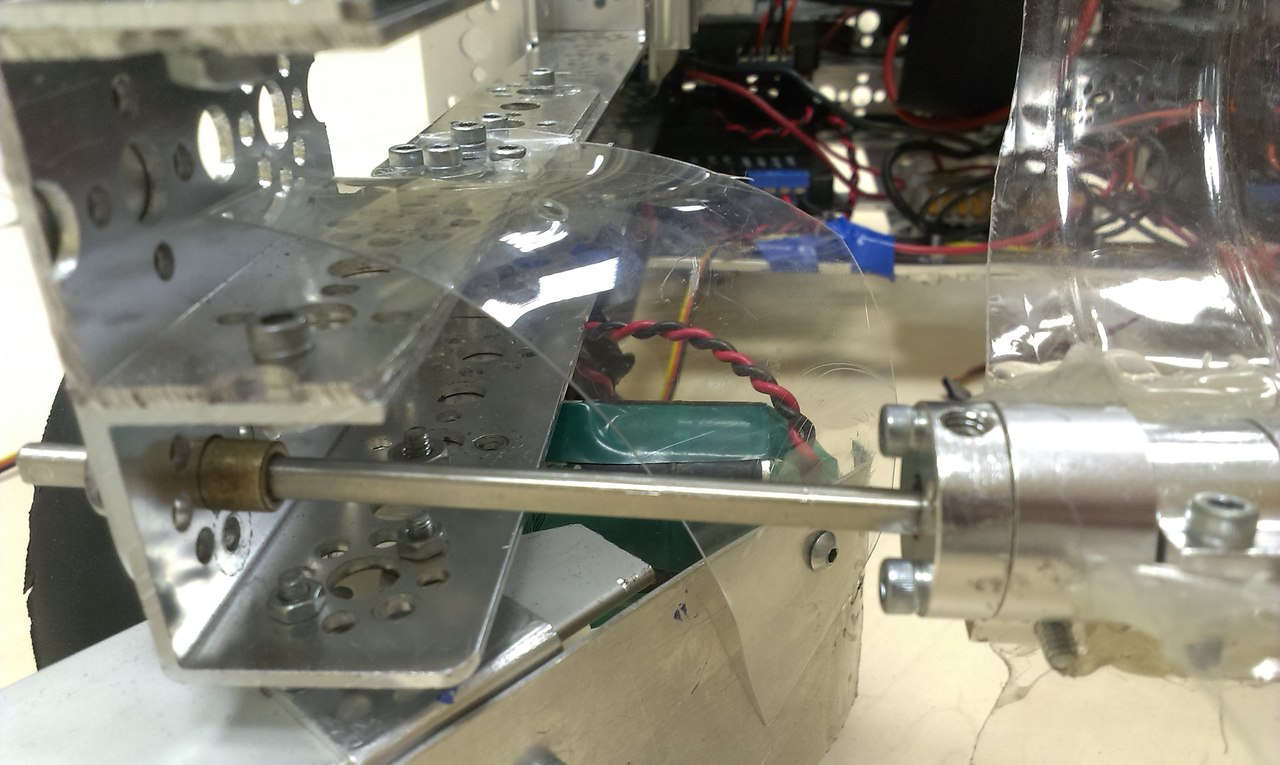
\includegraphics[scale=0.2]{days/22.12.14/images/01}}
	  		\caption{Новые откосы}
	  	  \end{minipage}
	   \end{figure}

	\end{enumerate}
	
	\item Итоги собрания:
	\begin{enumerate}
		
		\item Привод заменен, но не испытан.
		
		\item Откосы установлены и протестированы. Результат положительный.
		
	\end{enumerate}
	
	\item Задачи для последующих собраний:
	\begin{enumerate}
		
		\item Укрепить ось на нижней паре реек подъемника.
		
		\item Запаять концы проводов, соединяющих аккумулятор с драйверами.
		
		\item Испытать работоспособность нового привода.
		
	\end{enumerate}
\end{enumerate}
\fillpage
